% chapters/04_plan.tex
\chapter{开发计划}

\section*{本章开发计划速览}

\begin{table}[H]
    \centering
    \begin{tabular}{p{0.13\textwidth}p{0.18\textwidth}p{0.28\textwidth}p{0.25\textwidth}}
        \toprule
        \textbf{阶段} & \textbf{时间} & \textbf{核心内容} & \textbf{关键交付物} \\
        \midrule
        第一阶段 & 06-23 -- 06-28 & 用户态核心实现 & \texttt{dm} crate、单元测试、\texttt{dmctl} 工具 \\
        第二阶段 & 06-29 -- 07-10 & Linux 兼容性与工具链 & XTS 兼容验证、\texttt{cryptsetup} plain 模式 \\
        第三阶段 & 07-11 -- 07-20 & 内核补丁与 BIO 集成 & 补丁 0001--0004、rootfs 切换 \\
        第四阶段 & 07-21 -- 07-31 & 性能优化与基准框架 & 补丁 0005--0006、FIO 矩阵脚本 \\
        第五阶段 & 08-01 -- 08-11 & 组合栈与最终验证 & 补丁 0007、五轮性能矩阵、证据归档 \\
        第六阶段 & 08-09 -- 08-18 & 文档整合、答辩与收尾 & 两份 PDF、PPT、视频、最终 README \\
        \bottomrule
    \end{tabular}
\end{table}

\begin{figure}[H]
    \centering
    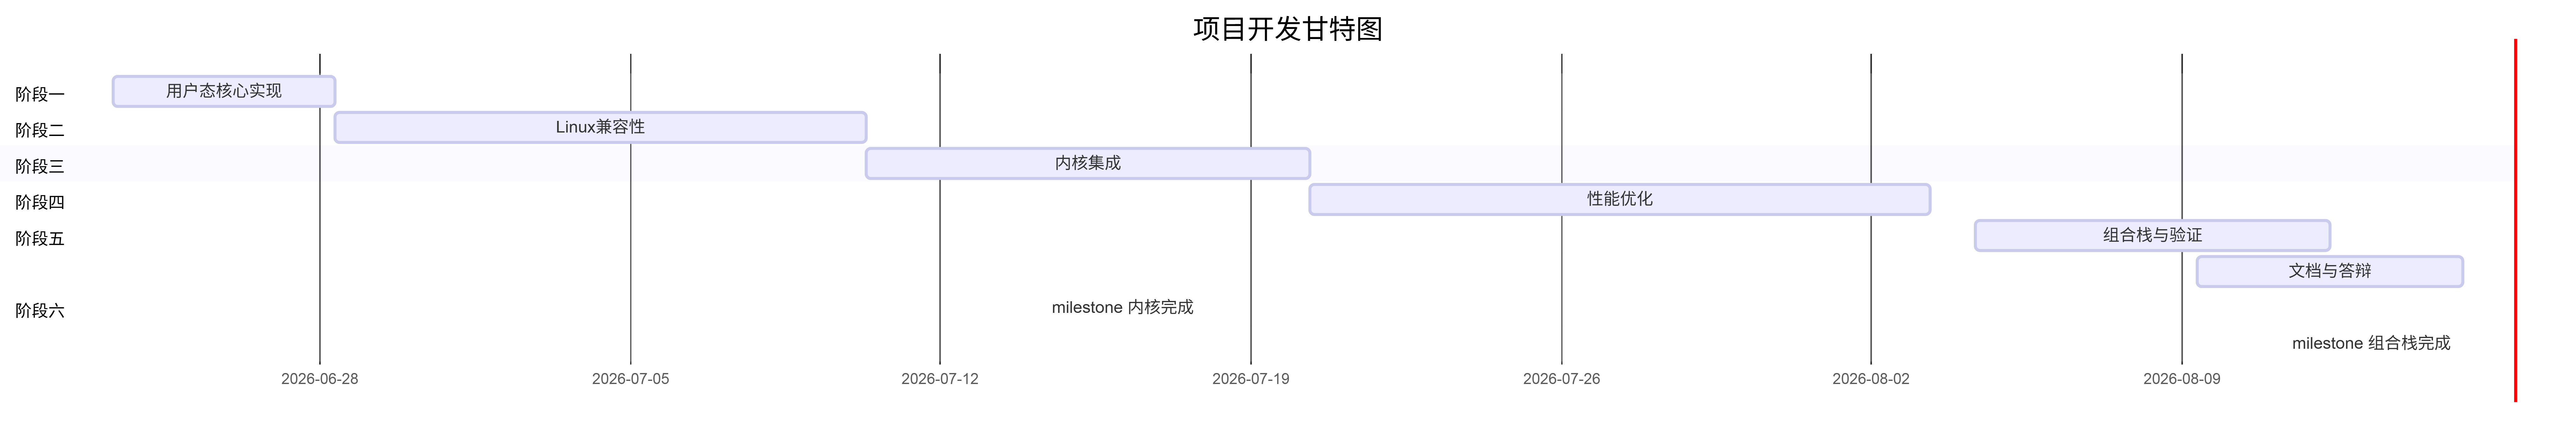
\includegraphics[width=1\textwidth]{development_gantt.png}
    \caption{项目开发甘特图（2026-06-23 至 2026-08-18，全程 57 天）}
    \label{fig:gantt}
\end{figure}

\section{开发方法论}

在制定开发计划时，我们遵循以下方法论原则，确保开发过程可控、可追溯：

\begin{enumerate}
    \item \textbf{先用户态后内核}：所有核心算法（AES-XTS、SHA-256、Merkle 树）先在用户态充分验证，再通过补丁序列接入内核。用户态作为"安全网"，可以在不依赖复杂内核环境的前提下快速迭代和调试；
    \item \textbf{每个补丁一个可验收增量}：补丁 0001：组件骨架与 target；0002：BIO / ext2 魔数自检；0003：\texttt{dm-root} + \texttt{pivot\_root}；0004：\texttt{dm\_ioctl}；0005：性能优化；0006：阶段归因；0007：组合栈。每一步都有明确的验收标准；
    \item \textbf{测完再优化}：正确性 PASS 后再跑正式 FIO；在优化之前先建立性能基准（五轮 FIO、Filebench、SQLite、启动耗时），优化措施的效果通过前后对比量化验证；
    \item \textbf{文档跟代码走}：每个阶段完成后同步更新技术文档和用户手册，避免"代码改完、文档滞后"的常见问题。
\end{enumerate}

上述方法论的核心可概括为\textbf{"先保证安全语义，再接入真实块路径，最后固化复现入口"}。这一原则贯穿了整个开发周期：在用户态用 \texttt{BlockDevice} 抽象验证 AES-XTS、Merkle 树与错误边界；通过 \texttt{VirtioBlkAdapter} 接入 Asterinas BIO，不绕过真实下层设备；分别完成 crypt、verity 与组合栈后，再接入受保护 rootfs；最终使用 Linux 兼容性、KVM 正反例和物理损坏测试作为合入门禁，性能数据必须通过 target、参数和完成语义审计。

\section{阶段划分与时间安排}

本项目实际开发周期为 2026 年 6 月 23 日至 8 月 18 日，共计 57 天，分为六个阶段。其中 08-12 至 08-18 为文档整合与收尾期，完成文档统一、答辩材料提交、表格修订与测试完善。以下按阶段详细描述计划内容与实际完成情况。

\section{第一阶段：用户态核心实现}

\subsection{目标}
在用户态完成 Device Mapper 核心逻辑，不依赖任何操作系统特定接口，使用 \texttt{MemoryBlockDevice} 和 \texttt{FileBlockDevice} 进行验证。这是整个项目的"地基"阶段。

\subsection{任务分解}
\begin{enumerate}
    \item 设计并实现 \texttt{BlockDevice} trait 及内存/文件后端；
    \item 实现 \texttt{sha256} 模块（纯 Rust，无外部依赖，约 120 行）；
    \item 实现 \texttt{hash\_tree} 模块（Merkle 树构建与验证，约 150 行）；
    \item 实现 \texttt{DmCryptDevice}（AES-256-XTS，使用 \texttt{aes} crate，约 350 行）；
    \item 实现 \texttt{DmVerityDevice}（只读完整性校验，约 200 行）；
    \item 实现 \texttt{DmStackBuilder}（可组合映射器链，约 180 行）；
    \item 编写单元测试覆盖核心场景（13+ 个测试）；
    \item 实现 \texttt{dmctl} 命令行工具的基础子命令（约 800 行）。
\end{enumerate}

\subsection{交付物与验收标准}
\begin{itemize}
    \item \textbf{交付物}：\texttt{\seqsplit{crates/dm/src/}} 全部核心模块；\texttt{\seqsplit{crates/dmctl/src/main.rs}} 基础命令
    \item \textbf{验收标准}：
    \begin{enumerate}
        \item \texttt{demo-crypt} 输出 \texttt{ciphertext\_differs: true}；
        \item \texttt{demo-verity} 输出 \texttt{tamper\_detected: true}；
        \item 所有单元测试 PASS。
    \end{enumerate}
\end{itemize}

\subsection{实际完成情况}
\begin{itemize}
    \item 完成时间：2026-06-23（Git commit \texttt{40a52179} \texttt{\seqsplit{feat: add Linux-compatible device mapper implementation}}）；
    \item 通过全部 13+ 个单元测试；
    \item \texttt{demo-crypt} 和 \texttt{demo-verity} 验证通过；
    \item 代码量：约 1500 行 Rust。
\end{itemize}

\section{第二阶段：Linux 兼容性与工具链}

\subsection{目标}
确保 AES-256-XTS 实现与 Linux 内核 \texttt{aes-xts-plain64} 逐字节兼容，并为 \texttt{cryptsetup} 工具提供控制接口。这是确保项目与 Linux 生态互操作的关键阶段。

\subsection{任务分解}
\begin{enumerate}
    \item 实现 \texttt{DmCryptTable} 解析器（支持 Linux table 格式，约 200 行）；
    \item 实现 \texttt{Aes256XtsCipher} 的 \texttt{plain64} IV 语义；
    \item 编写 \texttt{verify\_linux\_xts\_compat.sh} 交叉验证脚本；
    \item 实现 \texttt{/dev/mapper/control} 的 \texttt{dm\_ioctl} 兼容接口（\texttt{dm\_control.rs}，约 520 行）；
    \item 实现 \texttt{RuntimeMapper} 状态机（Empty、Loaded、Active，约 260 行）；
    \item 在 KVM 中验证 \texttt{cryptsetup open/read/close} 流程（R01）。
\end{enumerate}

\subsection{交付物与验收标准}
\begin{itemize}
    \item \textbf{交付物}：\texttt{DmCryptTable} 和 \texttt{\seqsplit{DmCryptDevice::from\_table}}；\texttt{\seqsplit{kernel/src/device/misc/dm\_control.rs}}；\texttt{\seqsplit{kernel/comps/dm/src/runtime.rs}}
    \item \textbf{验收标准}：
    \begin{enumerate}
        \item \texttt{verify\_linux\_xts\_compat.sh} 输出 \texttt{PASS}，SHA-256 匹配；
        \item KVM 中 \texttt{cryptsetup open/read/close} 全部 PASS。
    \end{enumerate}
\end{itemize}

\subsection{实际完成情况}
\begin{itemize}
    \item 完成时间：2026-07-14（补丁 0004）；
    \item Linux XTS 固定向量 SHA-256：\texttt{4334c17f...}；
    \item R01 cryptsetup smoke PASS（证据：\texttt{\seqsplit{R01-cryptsetup-persistent-cache.log}}）；
    \item 代码量：新增约 1000 行内核代码。
\end{itemize}

\section{第三阶段：内核补丁与 BIO 集成}

\subsection{目标}
将 \texttt{aster-dm} 组件完整接入 Asterinas 内核，支持启动参数解析、mapper 注册、BIO 处理和根文件系统切换。这是项目从"用户态玩具"走向"真实内核模块"的关键阶段。

\subsection{任务分解}
\begin{enumerate}
    \item 补丁 0001：组件骨架与 crypt/verity target、VirtIO 适配；
    \item 补丁 0002：BIO 路径与 ext2 魔数自检；
    \item 补丁 0003：\texttt{dm-root} + initramfs 挂载与 \texttt{pivot\_root} 切换；
    \item 补丁 0004：\texttt{dm\_ioctl} 控制面与 mapper 生命周期；
    \item 验证 dm-crypt 根文件系统启动（R02）；
    \item 验证 dm-verity 根文件系统启动（R03/V01）；
    \item 验证单字节篡改拒绝（V02--V07）。
\end{enumerate}

\subsection{交付物与验收标准}
\begin{itemize}
    \item \textbf{交付物}：\texttt{\seqsplit{asterinas\_port/patches/0001--0004.patch}}；\texttt{\seqsplit{tools/run\_dm\_crypt.sh}} 和 \texttt{\seqsplit{tools/run\_dm\_verity.sh}}
    \item \textbf{验收标准}：
    \begin{enumerate}
        \item R02 串口输出 \texttt{PASS system root switched to protected mapper}；
        \item R03/V01 串口输出 \texttt{status=verified} 和根切换 PASS；
        \item V02--V07 篡改后输出 \texttt{status=integrity-rejected}，无根切换 PASS。
    \end{enumerate}
\end{itemize}

\subsection{实际完成情况}
\begin{itemize}
    \item 完成时间：2026-07-14（补丁 0001--0004）；
    \item R01--R03、C01--C05、V01--V07 全部 PASS；
    \item 证据日志位于 \texttt{\seqsplit{docs/evidence/stabilization/correctness-kvm/}}；
    \item 补丁代码量：约 2500 行。
\end{itemize}

\section{第四阶段：性能优化与基准框架}

\subsection{目标}
实现性能优化（AES-NI、scratch pool、hash cache、BIO 复用），并建立可复现的五轮性能基准框架。本阶段的成果直接影响"性能与启动要求"指标的达成。

\subsection{任务分解}
\begin{enumerate}
    \item 补丁 0005：AES-NI 后端、scratch pool、hash cache、正式 benchmark 参数；
    \item 补丁 0006：性能阶段归因（\texttt{/proc/dm-performance-stats}）与正式合同；
    \item 实现 \texttt{scripts/run\_fio\_matrix.sh}（Linux QEMU virtio 与 Asterinas KVM 两平台）；
    \item 实现 Filebench、SQLite、启动耗时测试脚本；
    \item 完成 A/B 对比验证优化效果。
\end{enumerate}

\subsection{交付物与验收标准}
\begin{itemize}
    \item \textbf{交付物}：补丁 0005--0006；\texttt{\seqsplit{scripts/run\_fio\_matrix.sh}}、\texttt{\seqsplit{scripts/run\_filebench\_matrix.sh}}、\texttt{\seqsplit{scripts/run\_sqlite\_matrix.sh}}、\texttt{\seqsplit{scripts/run\_boot\_matrix.sh}}
    \item \textbf{验收标准}：
    \begin{enumerate}
        \item 五轮 FIO 矩阵可自动执行并生成 CSV；
        \item \texttt{dm.perf\_stats=1} 时阶段计时正常输出；
        \item 优化后 \texttt{data\_rereads=0}，\texttt{auth\_shortcuts} > 0。
    \end{enumerate}
\end{itemize}

\subsection{实际完成情况}
\begin{itemize}
    \item 完成时间：2026-08-03（补丁 0005--0006）；
    \item AES-NI 启动日志显示 \texttt{backend=AES-NI}；
    \item 正式性能矩阵于 2026-08-11 完成；
    \item 补丁代码量：约 800 行。
\end{itemize}

\section{第五阶段：组合栈与最终验证}

\subsection{目标}
实现 \texttt{dm-crypt $\to$ dm-verity} 组合栈（补丁 0007），完成全部性能基准测试并归档证据。这是项目从"单层保护"走向"组合保护"的最终形态。

\subsection{任务分解}
\begin{enumerate}
    \item 补丁 0007：\texttt{dm\_stack=crypt,verity} 启动路径；
    \item 实现 \texttt{scripts/build\_stack\_rootfs.sh} 和 \texttt{scripts/run\_dm\_stack.sh}；
    \item 完成 Linux QEMU virtio FIO 13+13 项（raw + dm-crypt）与 verity 读 7 项；
    \item 完成 Asterinas KVM FIO 13+7 项（dm-crypt + dm-verity 读）；
    \item 完成 Filebench、SQLite、启动耗时各 5 轮；
    \item 运行 \texttt{check\_benchmark\_package.py} 验证包完整性。
\end{enumerate}

\subsection{交付物与验收标准}
\begin{itemize}
    \item \textbf{交付物}：补丁 0007；\texttt{\seqsplit{scripts/build\_stack\_rootfs.sh}} 和 \texttt{\seqsplit{scripts/run\_dm\_stack.sh}}
    \item \textbf{验收标准}：
    \begin{enumerate}
        \item 组合栈串口输出 \texttt{stacked mapper: vdc -> dm-crypt0 -> dm-verity0}；
        \item 最终矩阵包含 46 个 PASS 单元格；
        \item \texttt{review\_release\_check.py} 全部通过。
    \end{enumerate}
\end{itemize}

\subsection{实际完成情况}
\begin{itemize}
    \item 完成时间：2026-08-11（补丁 0007，commit \texttt{6385e70b}）；
    \item 最终矩阵 46 PASS + 6 只读 N/A；
    \item 证据目录完整，\texttt{review\_release\_check.py} PASS；
    \item 补丁代码量：约 150 行（组合栈逻辑本身精简，复用已有 crypt/verity 实现）。
\end{itemize}

\section{第六阶段：文档整合、答辩与收尾}

\subsection{目标}
完成两份 PDF（设计赛道文档与技术文档）、答辩 PPT、演示视频的整理与提交，并完成 README 统一、表格修订与测试完善的收尾工作。

\subsection{任务分解}
\begin{enumerate}
    \item 设计赛道文档（\texttt{docs/design\_doc/}，10 章，严格按大赛大纲组织）；
    \item 技术文档（架构设计、模块说明、算法展开、合规与用户手册），两份 PDF 互为补充；
    \item 答辩 PPT（PPTX/PDF）与 8 分钟答辩视频；
    \item 演示视频（含运行环境介绍与受保护 rootfs 启动）；
    \item README 统一为十章策略版，性能表格核对修订；
    \item 测试代码注释完善与全量回归；
    \item AI 工具使用声明。
\end{enumerate}

\subsection{交付物与验收标准}
\begin{itemize}
    \item \textbf{交付物}：\texttt{\seqsplit{docs/design\_doc/design\_doc.pdf}}；技术文档 PDF；答辩 PPT（PPTX/PDF）；8 分钟答辩视频；演示视频；最终 README
    \item \textbf{验收标准}：
    \begin{enumerate}
        \item 所有文档可编译生成 PDF；
        \item 演示视频完整展示受保护 rootfs 启动；
        \item 性能表格与证据目录逐项核对一致；
        \item 全量测试通过；
        \item AI 工具声明完整披露工具名称、模型和使用场景。
    \end{enumerate}
\end{itemize}

\subsection{实际完成情况}
\begin{itemize}
    \item 08-18：两份 PDF、答辩 PPT 与 8 分钟视频定稿，PPT 与视频通过希冀专门入口提交，演示视频上传百度网盘（提取码 \texttt{oscp}）；
    \item 08-16 -- 08-17：README 补全用户态与内核态说明、256 MiB 正式合同与 Linux guest 对照表（\texttt{d56affa8}、\texttt{6e06b136}），技术文档重编并与 README 对齐（\texttt{7cd6d8f1}），设计文档整合（\texttt{9894d4bf}）；
    \item 08-18：FIO 表格修订为 qd=1 配置（\texttt{a0b7aacf}、\texttt{72f6738c}），测试注释完善，最终 README 更新（\texttt{ef345837}），全量测试通过（\texttt{b3247e0e}）。
\end{itemize}

\section{里程碑与关键交付物汇总}

\begin{table}[H]
    \centering
    \caption{关键里程碑与交付物}
    \label{tab:milestones}
    \begin{tabular}{p{0.12\textwidth}p{0.15\textwidth}p{0.55\textwidth}}
        \toprule
        \textbf{里程碑} & \textbf{日期} & \textbf{关键交付物} \\
        \midrule
        M1：用户态核心完成 & 06-23 & \texttt{dm} crate、\texttt{dmctl} 工具、单元测试 PASS（\texttt{40a52179}） \\
        M2：Linux 兼容性验证 & 07-10 & XTS 逐字节兼容证据、\texttt{/dev/mapper/control}（补丁 0004） \\
        M3：内核 rootfs 切换 & 07-14 & R01--R03、C01--C05、V01--V07 全部 PASS（补丁 0001--0004） \\
        M4：性能优化与框架 & 08-03 & AES-NI、scratch pool、hash cache、五轮 FIO 脚本（补丁 0005--0006） \\
        M5：组合栈与最终验证 & 08-11 & 补丁 0007、46 PASS 性能矩阵（\texttt{6385e70b}） \\
        M6：文档答辩定稿 & 08-18 & 两份 PDF、答辩 PPT、视频（希冀专门入口提交） \\
        M7：收尾完成 & 08-18 & README 统一、表格修订、测试全量通过（\texttt{b3247e0e}） \\
        \bottomrule
    \end{tabular}
\end{table}

\section{开发环境与工具链}

\begin{table}[H]
    \centering
    \caption{开发环境依赖}
    \begin{tabular}{p{0.20\textwidth}p{0.25\textwidth}p{0.45\textwidth}}
        \toprule
        \textbf{依赖项} & \textbf{版本要求} & \textbf{用途} \\
        \midrule
        Rust / Cargo & 1.75.0+ & 核心语言工具链（用户态） \\
        Asterinas 工具链 & \texttt{nightly-2026-04-03} & 星绽内核编译 \\
        QEMU & 8.2.2+ & 硬件虚拟化（KVM 加速，\texttt{-cpu host}） \\
        Docker & 29.4.3+ & 容器化构建环境（用于内核构建） \\
        星绽镜像 & \texttt{\seqsplit{asterinas/asterinas:0.18.0-20260618}} & 官方工具链和构建环境 \\
        Clang / LLVM & 18.0.0+ & 内核编译 \\
        fio & 3.36+ & I/O 性能基准测试 \\
        Filebench & 1.5-alpha3+ & 文件系统基准测试 \\
        SQLite & 3.45.1+ & 数据库基准测试 \\
        \bottomrule
    \end{tabular}
\end{table}

Ubuntu 24.04 上可通过以下命令安装基础依赖：
\begin{lstlisting}[basicstyle=\ttfamily\small, breaklines=true]
sudo apt update
sudo apt install -y build-essential clang lld qemu-system-x86 docker.io
\end{lstlisting}

Rust 工具链安装：
\begin{lstlisting}[basicstyle=\ttfamily\small, breaklines=true]
curl --proto '=https' --tlsv1.2 -sSf https://sh.rustup.rs | sh
rustup default stable
\end{lstlisting}

构建系统方面，用户态使用 Cargo workspace 进行构建和测试，内核态通过 \texttt{make kernel} + OSDK 在 Docker 容器中编译。版本控制使用 Git（托管于 GitLab），文档工具使用 \LaTeX 和 Microsoft PowerPoint。

\section{风险应对}

\begin{table}[H]
    \centering
    \begin{tabular}{p{0.20\textwidth}p{0.30\textwidth}p{0.40\textwidth}}
        \toprule
        \textbf{风险} & \textbf{影响} & \textbf{应对措施} \\
        \midrule
        AES-XTS 与 Linux 不兼容 & cryptsetup 无法互操作，影响赛题指标 2 & 提前编写交叉验证脚本（\texttt{verify\_linux\_xts\_compat.sh}），逐字节比对，迭代修正直到完全一致 \\
        Asterinas BIO 接口变化 & 内核集成延迟 & 使用固定上游基线，补丁隔离，降低对上游 API 变动的依赖 \\
        性能测试不稳定 & 结果不可复现，影响赛题指标 4 & 固定五轮、交替顺序、保留原始 JSON/CSV，报告中位数和标准差而非选择最好一轮 \\
        虚拟化环境差异 & 跨平台倍率误解 & 分平台展示，不计算跨环境倍率，Linux 作为参考对照而非性能标尺 \\
        缓存安全性削弱 & 完整性边界被突破，影响赛题指标 1 & "先认证后插入"设计原则，每个缓存块必须经完整 Merkle 路径验证才可插入，计数器（\texttt{auth\_shortcuts}）验证 \\
        容器拉依赖 & 构建失败或耗时过长 & 持久化 Cargo/rustup volume，预置 cryptsetup 到 initramfs，固定 Docker image digest \\
        \bottomrule
    \end{tabular}
\end{table}

\section{计划执行偏差分析}

实际开发与计划整体一致，仅有以下微调：

\begin{itemize}
    \item \textbf{第三阶段提前完成}：原计划 07-11 至 07-20，实际 07-14 完成，得益于用户态阶段的充分验证使内核集成更加顺利；
    \item \textbf{第四、五阶段合并执行}：性能优化与组合栈验证存在重叠，实际在 07-21 至 08-11 期间并行推进；
    \item \textbf{文档阶段与开发阶段重叠并延长}：技术文档的编写从第一阶段即开始；08-11 性能定稿后进入文档整合与收尾期（08-12 至 08-18），完成 README 统一、技术文档重编、答辩材料提交、FIO 表格修订与测试全量回归，最终于 08-18 关闭。
\end{itemize}

仓库 Git 提交覆盖完整周期（2026-06-23 至 2026-08-18），各里程碑对应的提交哈希已在各阶段"实际完成情况"与表 \ref{tab:milestones} 中记录，可逐一复核。按里程碑整理的提交时间线见图 \ref{fig:project_timeline}，08-11 性能定稿之后的提交列表见图 \ref{fig:git_history_5}--\ref{fig:git_history_7}。

\begin{figure}[H]
    \centering
    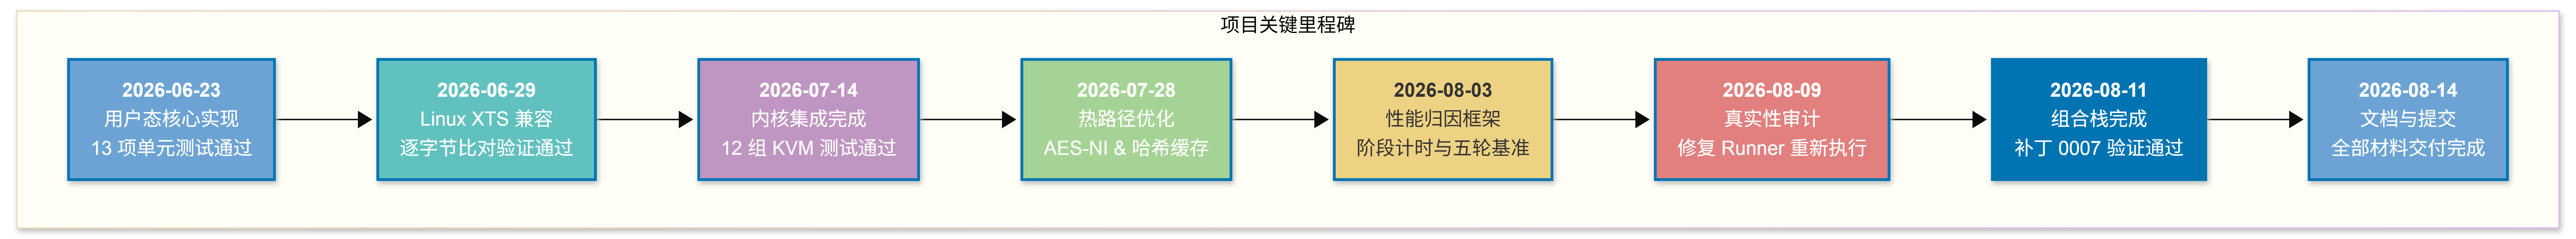
\includegraphics[width=1\textwidth]{project_timeline.png}
    \caption{项目提交时间线（2026-06-23 至 2026-08-18）}
    \label{fig:project_timeline}
\end{figure}

\begin{figure}[H]
    \centering
    \includegraphics[width=0.95\textwidth]{git_commit_history_5.png}
    \caption{GitLab 提交记录（2026-08-12 至 08-16）}
    \label{fig:git_history_5}
\end{figure}

\begin{figure}[H]
    \centering
    \includegraphics[width=0.95\textwidth]{git_commit_history_6.png}
    \caption{GitLab 提交记录（2026-08-17）}
    \label{fig:git_history_6}
\end{figure}

\begin{figure}[H]
    \centering
    \includegraphics[width=0.95\textwidth]{git_commit_history_7.png}
    \caption{GitLab 提交记录（2026-08-18）}
    \label{fig:git_history_7}
\end{figure}

\section{小结}

本章详细阐述了项目的开发计划，包括六个阶段的划分、任务分解、交付物、验收标准、实际完成情况、开发环境与工具链、风险应对和计划执行偏差分析。项目实际开发周期为 2026 年 6 月 23 日至 8 月 18 日，共计 57 天，完成了从用户态核心实现到内核集成、性能优化、组合栈验证、文档答辩与收尾的全流程。所有阶段均按计划完成，关键里程碑均有可复核的证据支撑，并由完整的 Git 提交记录佐证。

计划制定遵循"先用户态后内核、每个补丁一个可验收增量、测完再优化、文档跟代码走"的方法论，并贯穿"先保证安全语义，再接入真实块路径，最后固化复现入口"的研发原则，确保了开发过程的可控性和可追溯性。项目最终成果全面覆盖赛题五项技术指标，代码、证据、文档和演示材料均按大赛要求提交至指定托管平台。